\documentclass[12pt]{article}
\usepackage[english]{babel}
\usepackage{natbib}
\usepackage{url}
\usepackage[utf8x]{inputenc}
\usepackage{amsmath}
\usepackage{graphicx}
\graphicspath{{images/}}
\usepackage{parskip}
\usepackage{fancyhdr}
\usepackage{vmargin}
\setmarginsrb{3 cm}{2.5 cm}{3 cm}{2.5 cm}{1 cm}{1.5 cm}{1 cm}{1.5 cm}


							


\makeatletter
\let\thetitle\@title

\let\thedate\@date
\makeatother

\pagestyle{fancy}
\fancyhf{}
\rhead{\theauthor}
\lhead{\thetitle}
\cfoot{\thepage}

\begin{document}

%%%%%%%%%%%%%%%%%%%%%%%%%%%%%%%%%%%%%%%%%%%%%%%%%%%%%%%%%%%%%%%%%%%%%%%%%%%%%%%%%%%%%%%%%

\begin{titlepage}
	\centering
    \vspace*{0.5 cm}
    
\includegraphics[scale = 0.50]{IITB_logo.png}\\[1.0 cm]	% University Logo
    \textsc{\LARGE IIT BOMBAY}\\[2.0 cm]
    \textsc{\lARGE COMPUTER SCIENCE AND ENGINEERING}\\[0.2 cm]
    \textsc{\lARGE SOFTWARE LAB}\\[0.2 cm]
	\textsc{\Large CSE 699}\\[0.5 cm]				% Course Code
	\textsc{\large VOICE CONTROLLED EMAIL FOR VISUALLY IMPAIRED }\\[0.7 cm]
	\rule{\linewidth}{0.2 mm} \\[0.4 cm]
	
	\begin{centering}
	193050099 : Raj Krishna Srivastava\\
	193050059 : Vinod Kushwaha
	\end{centering}
	
	
\end{titlepage}

%%%%%%%%%%%%%%%%%%%%%%%%%%%%%%%%%%%%%%%%%%%%%%%%%%%%%%%%%%%%%%%%%%%%%%%%%%%%%%%%%%%%%%%%%

\tableofcontents
\pagebreak
%%%%%%%%%%%%%%%%%%%%%%%%%%%%%%%%%%%%%%%%%%%%%%%%%%%%%%%%%%%%%%%%%%%%%%%%%%%%%%%%%%%%%%%%%
\section{ABSTRACT}
Voice Based Email is an application which can be used by anyone to manage his mailbox through voice commands. Once the application starts the user can speak what he needs to do without using his hands or or eyes as the application will guide the user at each step through voice commands. The system will take the voice input from the user process the instructions and move to the next step accordingly.

\section{INTRODUCTION}
In today's world, the internet is something without which we cannot imagine our lives, from bringing groceries for the home, paying our bills to find a mate on matrimonial sites. For everything, we are dependent on the web. One very important aspect that has been revolutionized by modern-day technology is communication.  But what about people who cannot take advantage of this. Although many advancements have been made in this field too with a braille keyboard and other tools, all that requires prior training. In this project, we aim to develop an email-based system which can be used even by the visually challenged. The system will work only on mouse operation and speech recognition.


\section{MOTIVATION}
It is rightly said that necessity is the mother of all invention. The mother for this project was to make this a bit easier for visually impaired person. Enable him to access the internet and make use of it like a normal person would do. This is just a small step in that direction as our project will enable him to access his mails with ease.

\section{FEATURES}
1.Compose and Send Mails.\newline
2.Read Inbox.\newline
3.Delete Mails or Save to Drafts.\newline
4.Reply or Forward.
\pagebreak
\section{User Documentation}
\subsection{Flowchart}
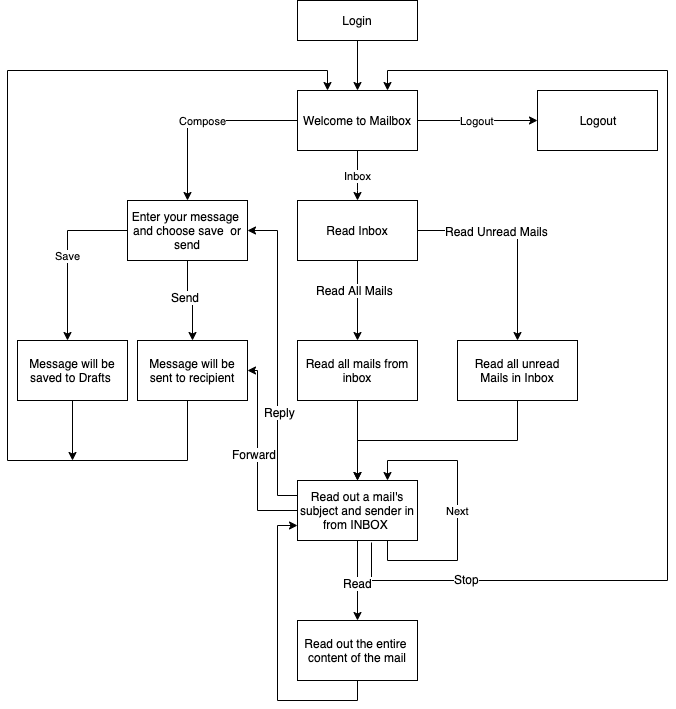
\includegraphics[height=18cm,width=16cm]{Flowchart.png}
\pagebreak
\subsection{Detailed Instruction}
\subsubsection{Login}
This is the very first step. The users login credentials are fetched from a file stored in a system. We assume that the system is not used by multiple users as normally is the case.
\subsubsection{Mailbox Home}
Once the user logs in he enters him Mailbox home. He gets three options here. \begin{itemize}
    \item Compose Mail
    \item Go to Inbox
    \item Logout
\end{itemize}
\subsubsection{Compose Mail}
The user has to speak in his message. And the email address of the recipient
Here the user get two options. \begin{itemize}
    \item Send : To send the mail to desired recipient
    \item Save : To save mail to draft
\end{itemize}

\subsubsection{Inbox}
Here the user gets option to check his inbox. All the mail subjects and sender are read out to the user after which he can choose on of the following options. \begin{itemize}
    \item Read : To read the entire message
    \item Reply : To reply to the current mail
    \item Forward : To forward the current mail
    \item Next : To read the next mail
    \iteam Stop : To stop reading mails from inbox
\end{itemize}

\section{Implementation}
The project is divided mainly into two modules.
\subsection{Text-Voice Handling}
\subsubsection{Speech to text}
This was on of the core parts of the project. The success of this application depends on how well this module is implemented. We used Google's speech\_recognition library to convert the command and messages taken through mike, to text. It is an open-source library and on one of the best speech recognizer for English language.\newline
We improved over this by calculating the weighted edit distance between all the available command at a given stage and the command recognized by speech recognition library. And it treats the input as the closest distance command option available at that stage provided the distance is less than a threshold \newline
Foe example, if a user says has four option after a mails subject and recipient are read out: Reply, Forward, Next, Stop and Read. Now the user gives an input which is recognized by google's speech recognition as 'top', in this case as it is quite certain that the user said stop. So the application will consider the input as stop as its distance to stop is least and less than the threshold, and act accordingly.
\subsubsection{Text to Speech}
Text to speech conversion is required to give commands and guide a blind user and he s unable to see anything on the screen. For converting text to speech we imported gtts library.
We saved the audio generated by gTTS and played it using mpg321.

\subsection{Sending and Retrieving Emails}
\subsubsection{Sending Mails}
For sending emails we have use 'smtplib'. Once the message is composed, to send the mail following steps are there. We establish the connection(TLS) with gmail's smtp server at port 587. Using the login and the password the user is authenticated. Finally the mail is Pushed to the users mailbox through SMTP protocol.
\subsubsection{Retrieving Mails}
Emails are retrieved from the users mailboc through IMAP or POP3. Here we use imaplib to retrieve emails. It is used to fetch all the mails in inbox , sent box or draft and bring it on the users system. The users login credentials are use to fetch these information from the server.  
.\newline

\section{RESULT}
Using the Voice Based Email application we are able to compose and send mail. We can also browse through the inbox, reply to mails, forward it to other recipient. Given the great quality speech recognition the system works quite well and very rarely gives an unexpected behavior.

\section{FUTURE SCOPE}
Future work will build upon adding addition features the email application and making it more user friendly and smooth while handling. Additional features can be giving options to add reminders, searching mails in inbox, saving the mails automatically. Adding a Braille keyboard with the system and using a combination of Braille keyboard and voice inputs can greatly improve the performance and ease of usability of the application. 


\section{CONCLUSION}
Voice Bases Email is an example of how by using the simple bits of knowledge, we can make something really useful and life for others.  In this project we have developed an application to make the email easily accessible to the visually impaired. A number of problem face by the would be solved with this. Eliminating the use of screen keyboards and screen readers while managing emails will greatly reduce the cognitive load of remembering keyboard shortcuts. Also no training is required to a naive user as interacting in this method is almost similar to talking to another person an instructing him/her to send or read your mail. The user only needs to follow the instruction given by the system. 


\end{document}
